\documentclass{standalone}
\usepackage{tikz}
\usepackage{ctex,siunitx}
\usepackage{tkz-euclide}
\usepackage{amsmath}
\usetikzlibrary{patterns, calc}
\usetikzlibrary {decorations.pathmorphing, decorations.pathreplacing, decorations.shapes,}
\begin{document}
\small
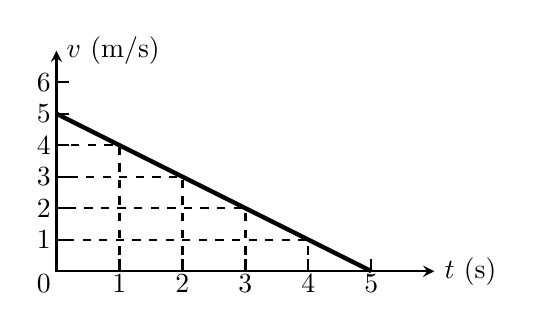
\begin{tikzpicture}[>=stealth, thick,scale=0.8]
  \draw [<->](0,3.5)node[right]{$v$ (\unit{m/s})}--(0,0)--(6,0)node[right]{$t$ (\unit{s})};
  \foreach \x in {1,2,...,5}
  {
      \draw(\x, 0) --(\x, .2);
      \node at (\x,-.2){$\x$};
  }
  \foreach \y in {1,2,3,...,6}
  {
      \draw(0,\y/2)--(.2, \y/2);
      \node at (-.2, \y/2){$\y$};
  }
  \node at (-.2,-.2){$0$};
  \draw [ultra thick](5,0)--(0,5/2) ;
  \foreach \z in{1,2,3,4}
  {
     \draw [dashed] (\z,0)--(\z, 2.5-\z/2)--(0, 2.5-\z/2);
  }
  %\node at (3,-1){$v_0=5{\rm m/s},\quad a=-1{\rm m/s}^2$};
\end{tikzpicture}
\end{document}